% arara: lualatex
% !TEX TS-program = LuaLaTeX

\documentclass{coderdojo}


\worksheet{4}{Some More Turtle Graphics}

\begin{document}
\maketitle


\section*{Introduction}

In this worksheet we will revisit turtle graphics basics to make sure that you are happy with the main ideas and cover some aspects of turtle graphics that we skipped over last week. So this week we will look at 


\begin{dingautolist}{192}
\item \hyperref[sec:spiral]{\color{section}\bfseries Generating Spirals using Turtle Graphics}

We will start with a simple turtle graphics program that generates a spiral and add then pimp it up, with colour and changing number of slides and line width.
 
 
\item \hyperref[sec:fill]{\color{section}\bfseries To Fill or Not Fill --- That is the Question}

So far all shapes have only drawn using their outline.  We now want to see about filling these shapes in. 


\item \hyperref[sec:tasks]{\color{section}\bfseries Practice makes perfect}

Finally we will end with some sample diagrams constructed using turtle commands.
 
\end{dingautolist}

\centerline{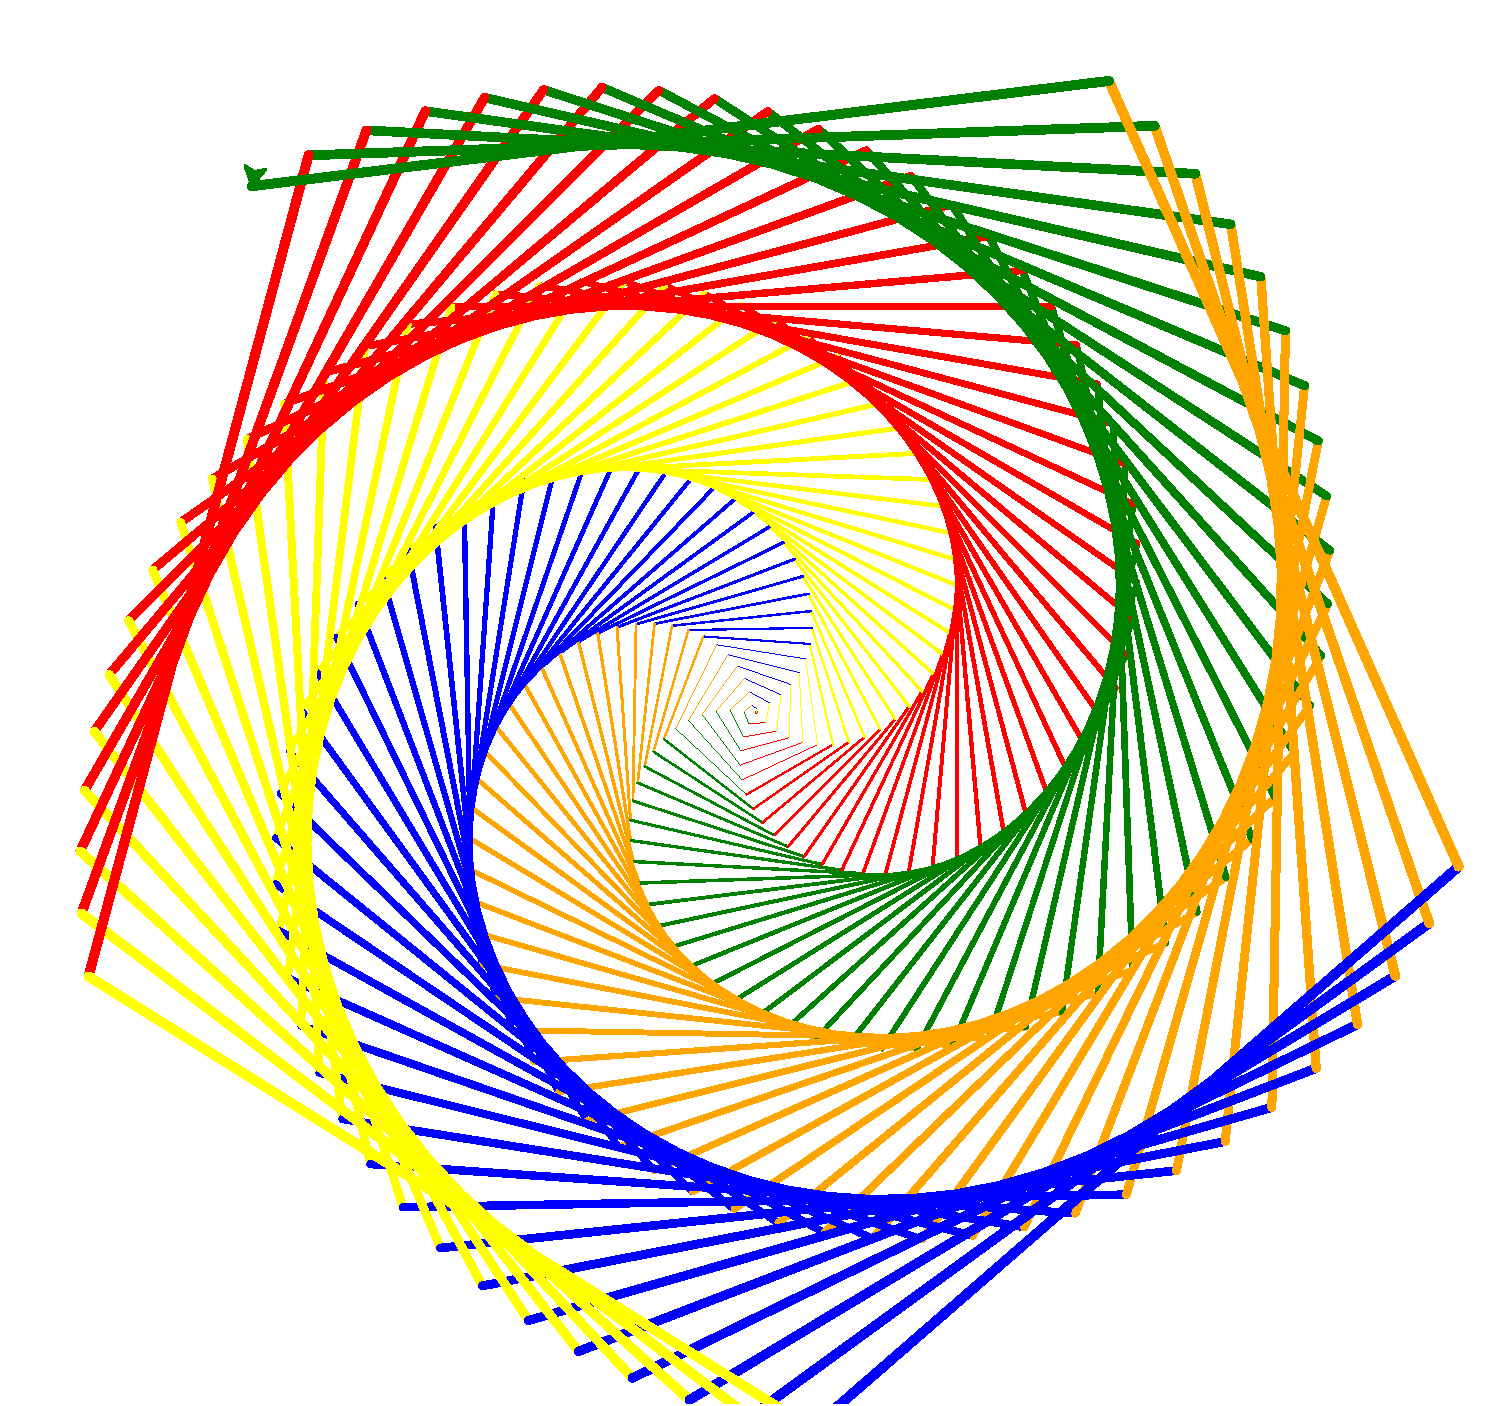
\includegraphics[clip,trim=0 0 0 0, width=.4\textwidth]{code/Color_Spiral_d.pdf}}
 
\clearpage

\section{A Simple Turtle Program}\label{sec:spiral}

\begin{itemize}
\item[\todoSymbol] \color{todo}
Create a new file with the following code and save as \code{Square_Spiral_1.py}.
\end{itemize}

\codeandoutput{title={\code{Square_Spiral_1.py}}}{1}{200}{code}{Square_Spiral_1.py}{%
	\centering	
	\tikz\node[fill=white]{
	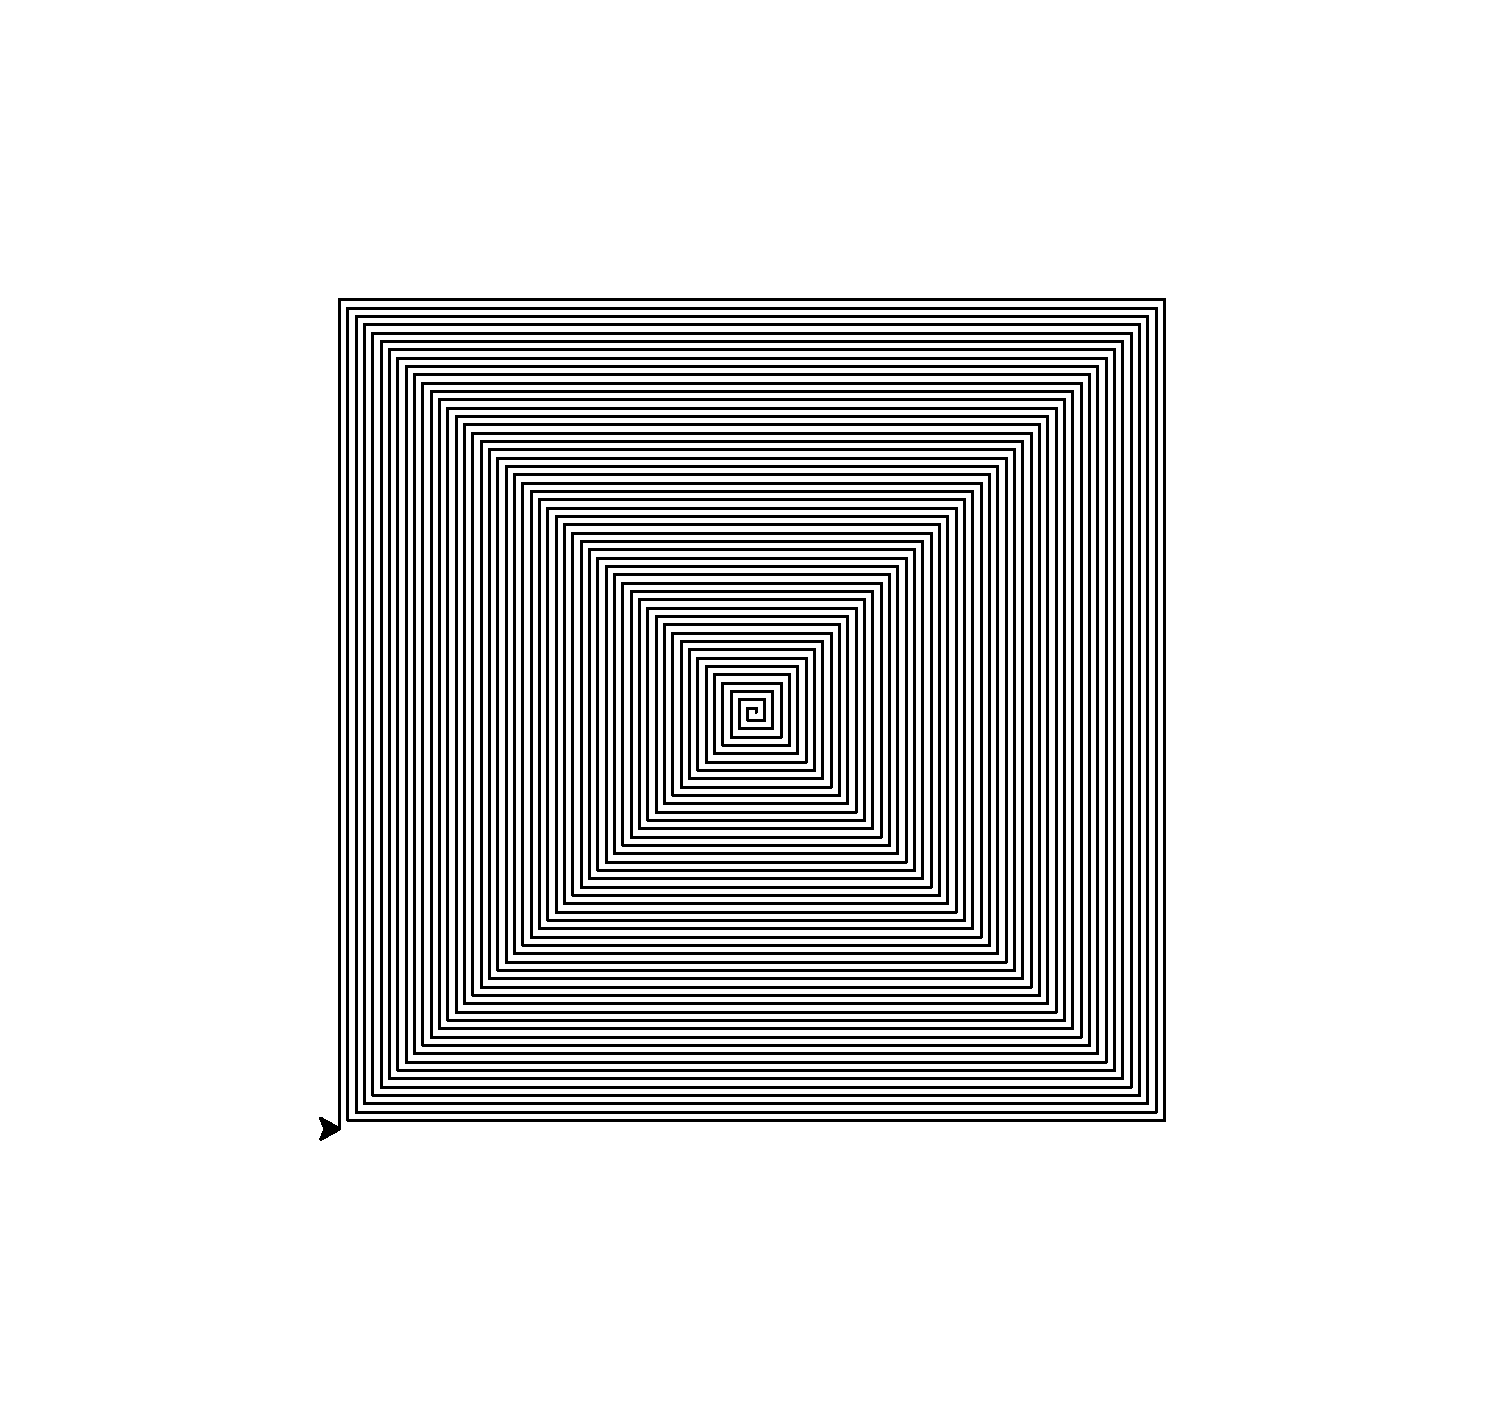
\includegraphics[clip,trim=70 70 70 70, width=\textwidth]{code/Square_Spiral_1.pdf}};
}

\subsection{How it works}

Let's break the program down line by line to see how it works.

\begin{itemize}

\item[{\smaller line 1:}]

The first line of \code{Square_Spiral_1.py} is a comment. A comment begins with a hash mark (\code{\#}). Comments allow us to write notes in our programs to ourselves or to other humans who might read the program later. The computer doesn't read or try to understand anything after the hash mark; the comment is just for us to write something about what the program is doing. In this case, I've put the name of the program in the comment, as well as a brief description of what it does.

\item[{\smaller line 3:}]

The next line of code gives us the ability to draw turtle graphics. 

Importing code that's already been written is one of the coolest things about programming. If you program something interesting and useful, you can share it with other people and even reuse it yourself. Some cool Python programmers built a library---a reusable set of code---to help other programmers use turtle graphics in Python.
When you type

\codeonly{}{3}{3}{code}{Square_Spiral_1.py}

you are saying that you want your program to be able to use the code that those Python programmers wrote. The little black arrow in represents the turtle, drawing with its pen as it moves around the screen.

\item[{\smaller line 3:}]

The next line of our program,

\codeonly{}{5}{5}{code}{Square_Spiral_1.py}

tells the computer to create a new turtle called \code{bob}.  By sending \code{bob} commands we can move \code{bob} and change it properties, such as colour and size.

\item[{\smaller line 7:}]

The next line is the most complex. Here we?re creating a \code{for} loop, which repeats a set of instructions a number of times (it loops through those lines of code over and over again). This particular loop sets up a range, or list, of 200 numbers from 0 to 199. (Computers almost always start counting at 0, not 1 like we usually do.) The loop then steps the letter \code{x} through each of the numbers in that range. So \code{x} starts as 0, and then it becomes 1, then 2, and so on as it counts all the way up to 199, for a total of 200 steps.

This \code{x} is called a {\bf loop variable}.  A variable stores a value that can change, or vary, as we move through our program. We'll be using variables in almost every program we write, so it's good to get to know them early.

\item[{\smaller lines 8\&9:}]
The next two lines are indented, or spaced over from the left. That means that they are in the loop and go with the line above, so they'll be repeated each time  \code{x} gets a new number in the range from 0 to 199, or 200 times.

\end{itemize}

\subsection{So what happens?}
	
Let's see what happens the first time Python reads this set of instructions. The command 

\codeonly{}{8}{8}{code}{Square_Spiral_1.py}

tells the turtle to move forward \code{2*x} dots on the screen. Because \code{x} is 0, the pen doesn't move at all. The last line, 

\codeonly{}{9}{9}{code}{Square_Spiral_1.py}

tells the turtle to turn left by 90 degrees, or a quarter turn.

Because of the \code{for} loop, the program continues to run, and it goes back to the starting position of our loop. The computer adds 1 to variable \code{x} to the next value in the range, and since 1 is still in the range from 0 to 199, the loop continues. Now \code{x} is 1, so the turtle moves forward 2 dots. The turtle then moves again to the left by 90, because of \code{bob.left(90)}. This continues again and again. By the time \code{x} gets to 199, the last time through the loop, the turtle is drawing the long lines around the outside of the square spiral.

\newcommand\tmp[1]{\\\mbox{}\hfill\raisebox{0pt}[24pt][24pt]{{\tikz\node[draw,fill=white,drop shadow]{\includegraphics[width=3cm,clip,trim=300 300 300 300]{Square_Spiral_1_#1}};}}}
\begin{description}
\item[After one iterations:] 
\parbox[t]{9cm}{(This is a fancy way of saying at the start!) We have done nothing yet so all we see is bob the turtle.}
\tmp{0}

\item[After iterations 0 to 4:] 
\parbox[t]{9cm}{The first four lines (the first line is tiny) are drawn (and now \code{x} stores 4).}
\tmp{4}

\item[After iterations 0 to 8:] The first 8 lines are drawn (and now \code{x} stores 8).
\tmp{8}

\item[After iterations 0 to 16:] The first 16 lines are drawn (and now \code{x} stores 16).
\tmp{16}

\end{description}

The dots, or pixels, on your computer screen are probably too tiny for you to see them very well. But, as \code{x} gets closer to 200, the turtle draws lines consisting of more and more pixels. In other words, as \code{x} gets bigger, \code{bob.forward(x)} draws longer and longer lines.

The turtle arrow on the screen draws for a while, then turns left, draws some more, turns left, and draws again and again, with longer lines each time.

By the end, we have a hypnotising square shape. Turning left 90 degrees four times gives us a square, just like turning left four times around a building will take you around the building and back where you started.

The reason we have a spiral in this example is that every time we turn left, we go a little farther. The first line that's drawn is just 2 dots long (when \code{x = 1}), then 4 (the next time through the loop), then 6, then 8, and so on, all the way through 200 steps, when the line is 398 pixels long. Again, the pixels are probably so tiny on your screen that you can't easily see the individual dots, but they're there, and you can see the lines get longer as they contain more pixels.

\subsection{Let's Turn Things a Bit \ldots}

Let's see what happens when we change one of the numbers in the program. One way to learn new things about a program is to see what happens when you change one part of it. You won't always get a pretty result, but you can learn even when something goes wrong.


\begin{itemize}
\item[\todoSymbol] \color{todo}
Create a new file with the following code and save as \code{Square_Spiral_2.py}.
\end{itemize}

\codeandoutput{title={\code{Square_Spiral_2.py}}}{1}{200}{code}{Square_Spiral_2.py}{%
	\centering	
	\tikz\node[fill=white]{
	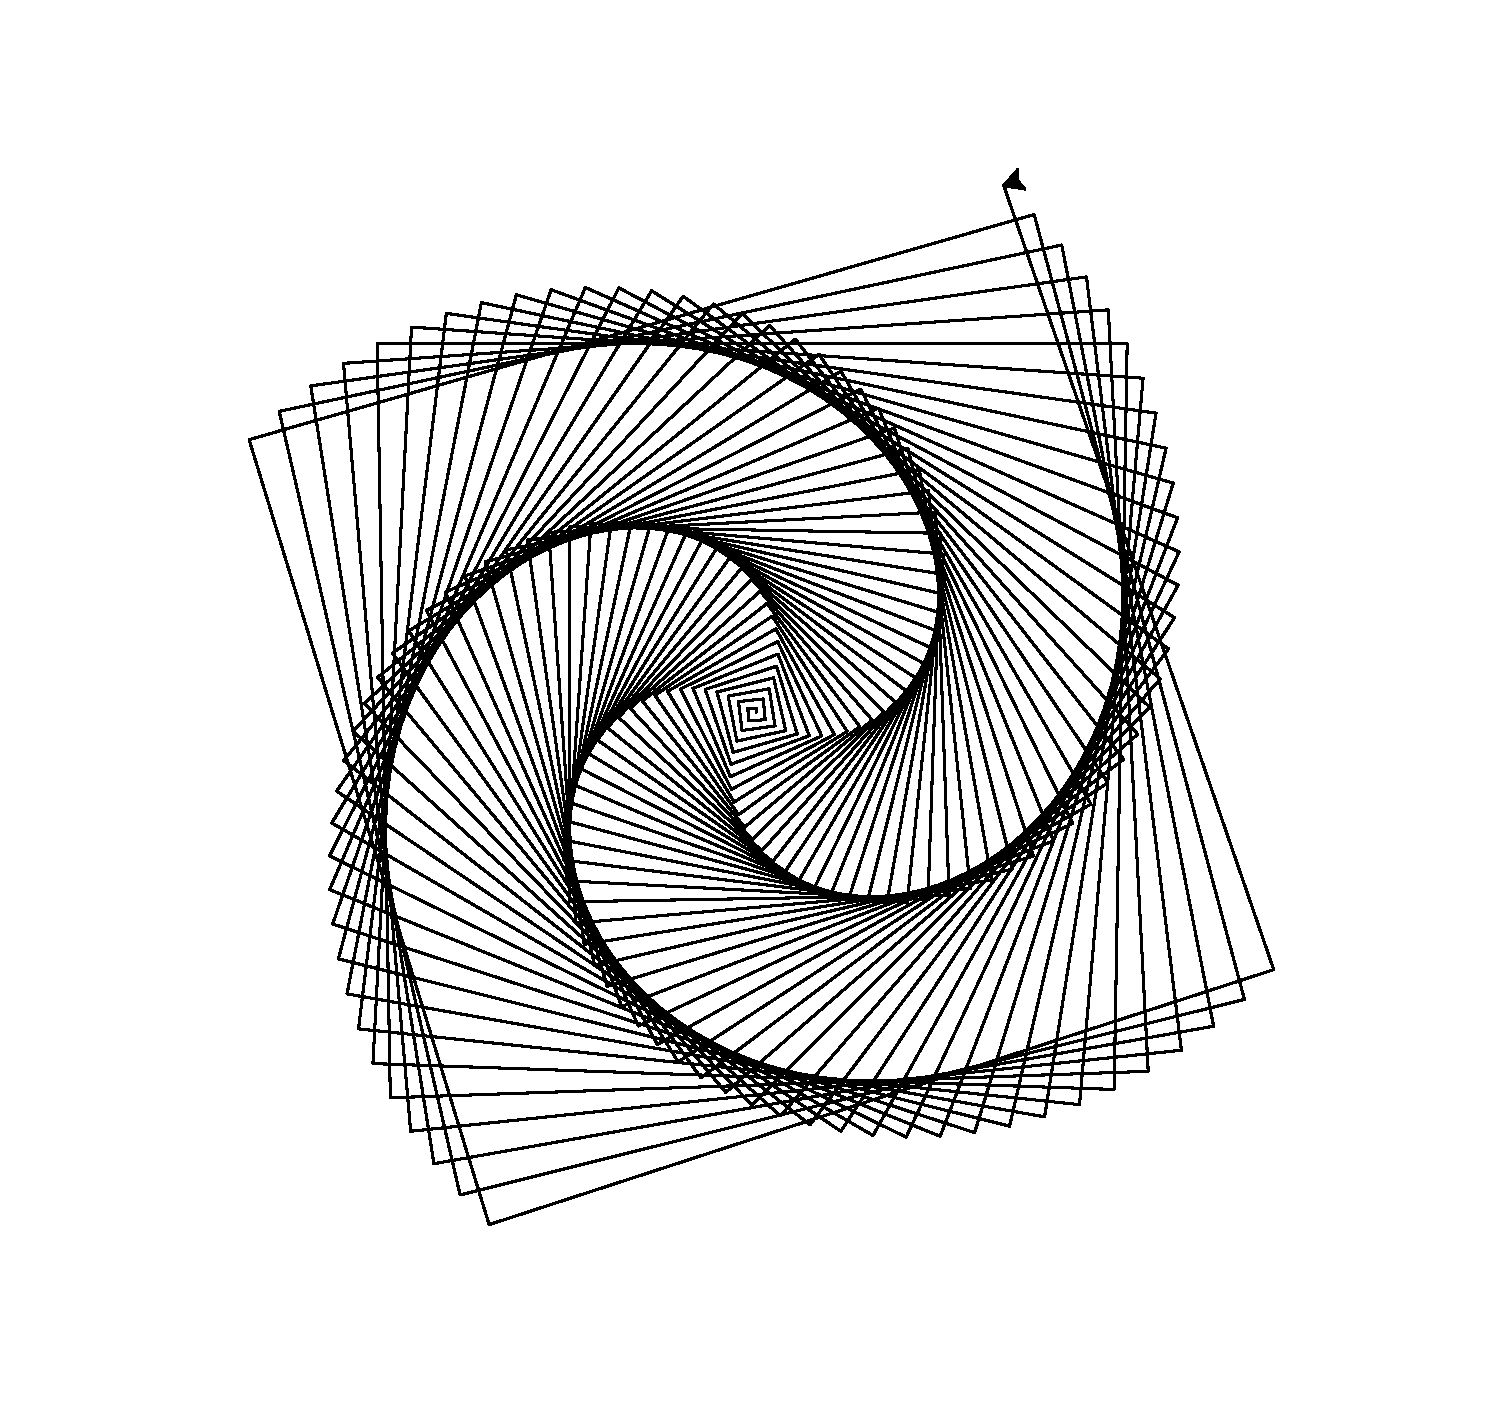
\includegraphics[clip,trim=70 70 70 70, width=\textwidth]{code/Square_Spiral_2.pdf}};
}

All we did was to change the last line of the program from  \code{bob.left(90)} to \code{bob.left(91)}.

Making a 90-degree left turn creates a perfect square. Turning just a little more than 90 degrees --- in this case, 91 degrees every turn --- throws the square off just a bit. And because it's already off a bit when it makes the next turn, our new shape looks less and less like a square as the program continues. In fact, it makes a nice spiral shape that starts to swirl to the left like a staircase, as you can see in .

%The square spiral program with one tiny change becomes a spiral staircase.

This is also a nice visual to help you understand how being off by just one number can drastically change the result of your program. One degree doesn't seem like a big deal, unless you're off by one degree 100 times (which adds up to 100 degrees), or 1,000 times, or if you're using a program to land an airplane \ldots


\begin{itemize}
\item[\todoSymbol] \color{todo}
If you don?t know how degrees work yet, don?t worry about it for now. Just play with the numbers and see what happens. 
\item
How can we change the size of the spiral?
\item 
How can we change the space between the lines in the spiral?
\item
How can we change the space between the lines in the spiral without changing the overall size?
\end{itemize}

\subsection{Don't be a square}

Turtle graphics can draw lots more interesting shapes than just straight lines. We'll come back to the square shape again in the next section, but let's take a short detour to check out more of the Python Turtle library.

Let's change one more line of code: \code{bob.forward(2*x)}. We saw earlier that this command moves the turtle forward \code{x} pixels and draws a straight line segment; then the turtle turns and does it again. What if we changed that line of code to draw something more complex, like a circle'

Fortunately for us, the command to draw a circle of a certain size, or radius, is as simple to code as the command to draw a straight line. Change \code{bob.forward(2*x)} to \code{bob.circle(x)}, as shown in the following code.

\codeandoutput{title={\code{Circle_Spiral_1.py}}}{1}{200}{code}{Circle_Spiral_1.py}{%
	\centering	
	\tikz\node[fill=white]{
	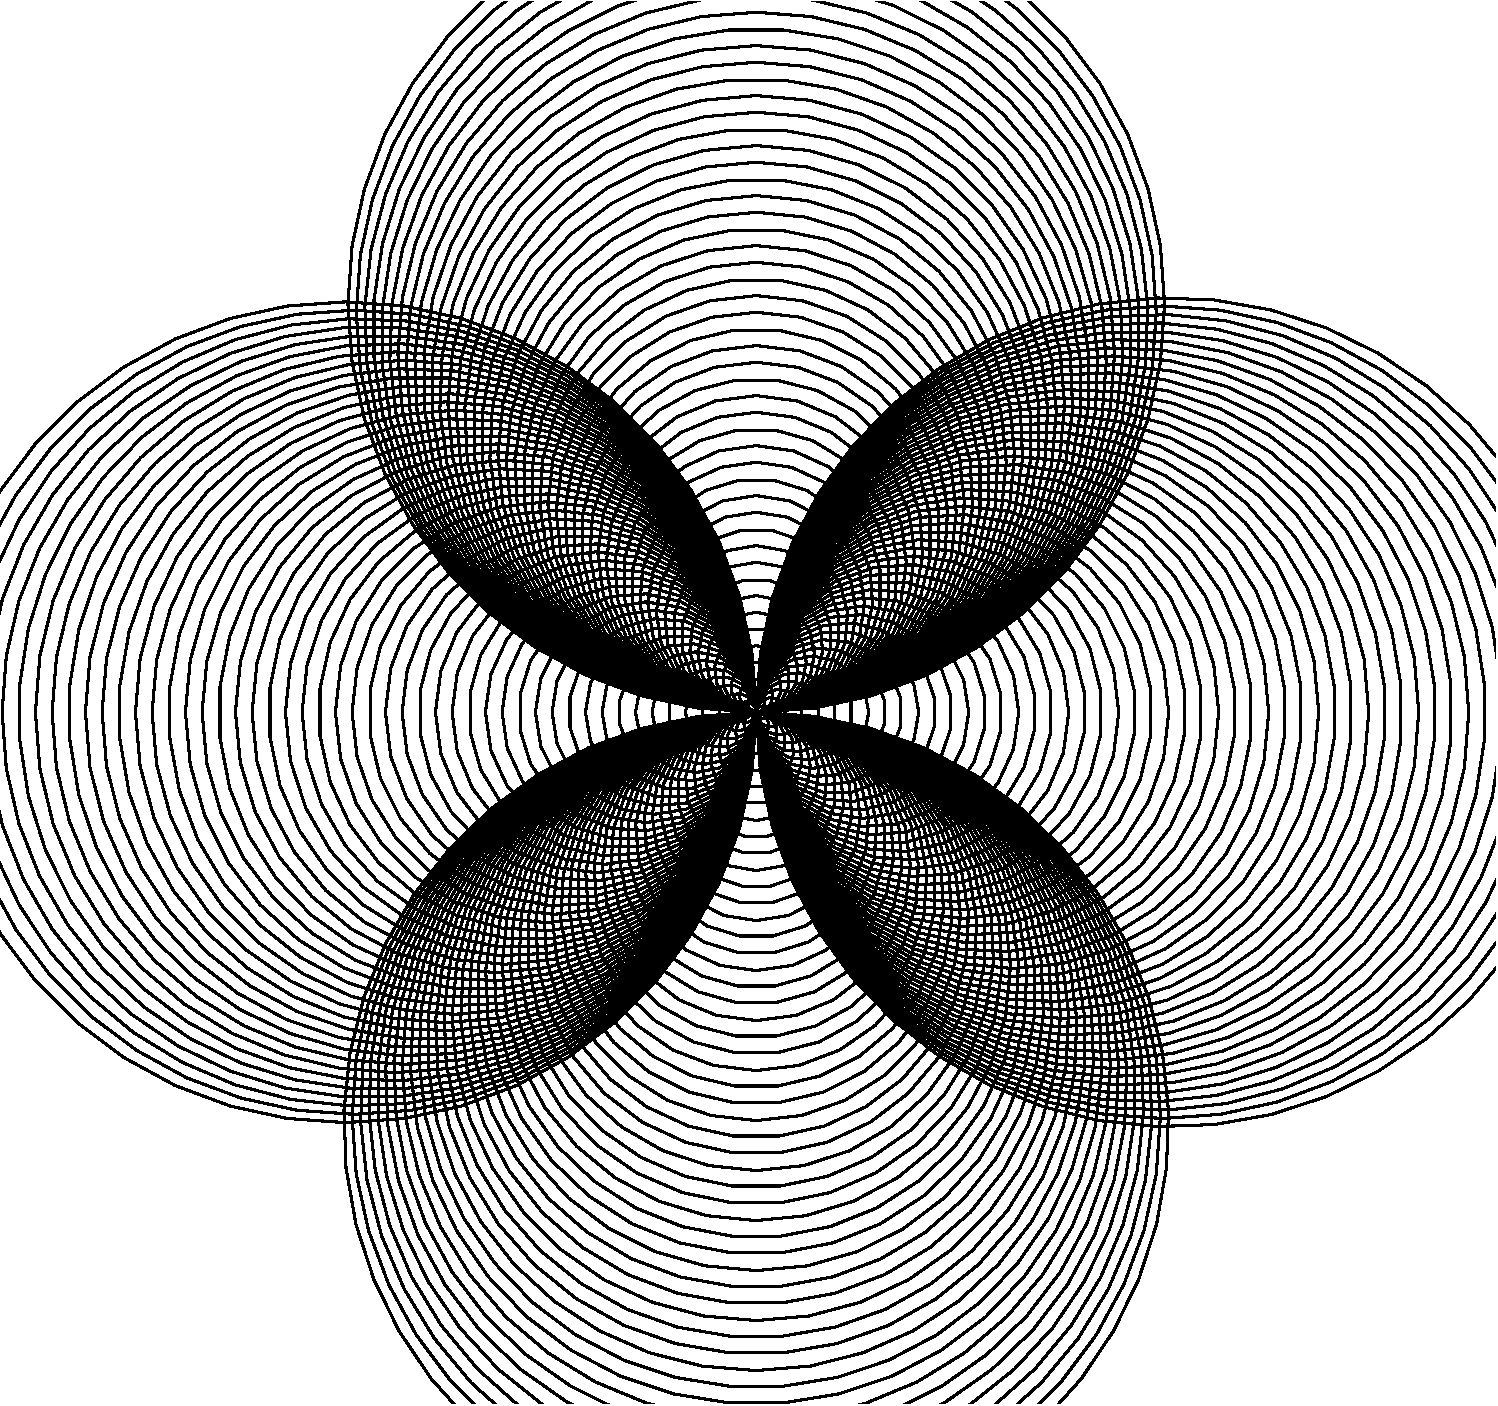
\includegraphics[clip,trim=0 0 0 0, width=\textwidth]{code/Circle_Spiral_1_fast.pdf}};
}


Changing one command from \code{bob.forward} to \code{bob.circle} gave us a much more complex shape, as you can see in . The \code{bob.circle(x)} function tells the program to draw a circle of radius \code{x} at the current position. Notice that this drawing has something in common with the simpler square spiral shape: there are four sets of circle spirals just like there were four sides to our square spiral. That's because we're still turning left just a little over 90 degrees with the \code{bob.left(91)} command. If you've studied geometry, you know that there are 360 degrees around a point, like the four 90-degree corners in a square (\(4 \times 90 = 360\)). The turtle draws that spiral shape by turning just a little more than 90 degrees each time around the block.

%One difference you'll see is that the circle spiral is larger than the square spiral ' about twice the size, in fact. This is because t.circle(x) is using x as the radius of the circle, which is the distance from the center to the edge, or one-half of the circle's width.

%A radius of x means that the diameter, or total width, of the circle will be two times x. In other words, t.circle(x) draws a circle 2 pixels across when x is equal to 1, 4 pixels across when x is 2, all the way up to 198 pixels across when x is 99. That's almost 200 pixels across, or twice the size of our biggest side in the square, so the circle spiral is about double the size of our square spiral ' and maybe twice as cool, too!

\begin{itemize}
\item
We have removed the multiplication by two in the drawing of a circle but the shape is still as large as before (in fact it is larger) Why?

Think radius versus diameter of a circle.

A radius of \code{x} means that the diameter, or total width, of the circle will be two times \code{x}. In other words, \code{bob.circle(x)} draws a circle 2 pixels across when \code{x} is equal to 1, 4 pixels across when x is 2, all the way up to 398 pixels across when x is 199. 
%That's almost 400 pixels across, or twice the size of our biggest side in the square, so the circle spiral is about double the size of our square spiral ' and maybe twice as cool, too!
\item
Also drawing a circle is very slow. so consider speeding up bob by using the command

\codeonly{}{6}{6}{code}{Circle_Spiral_1_fast.py}
\end{itemize}

\subsection{Adding a touch of colour}

These spirals are nice shapes, but wouldn't it be cooler if they were a bit more colourful? Let's go back to our square spiral code and add one more line to our program, right after the 
\code{bob = turtle.Turtle()} line, to set the pen colour to red:

\begin{itemize}
\item[\todoSymbol] \color{todo}
Create a new file with the following code and save as \code{Square_Spiral_3.py}.
\end{itemize}

\codeandoutput{title={\code{Square_Spiral_3.py}}}{1}{200}{code}{Square_Spiral_3.py}{%
	\centering	
	\tikz\node[fill=white]{
	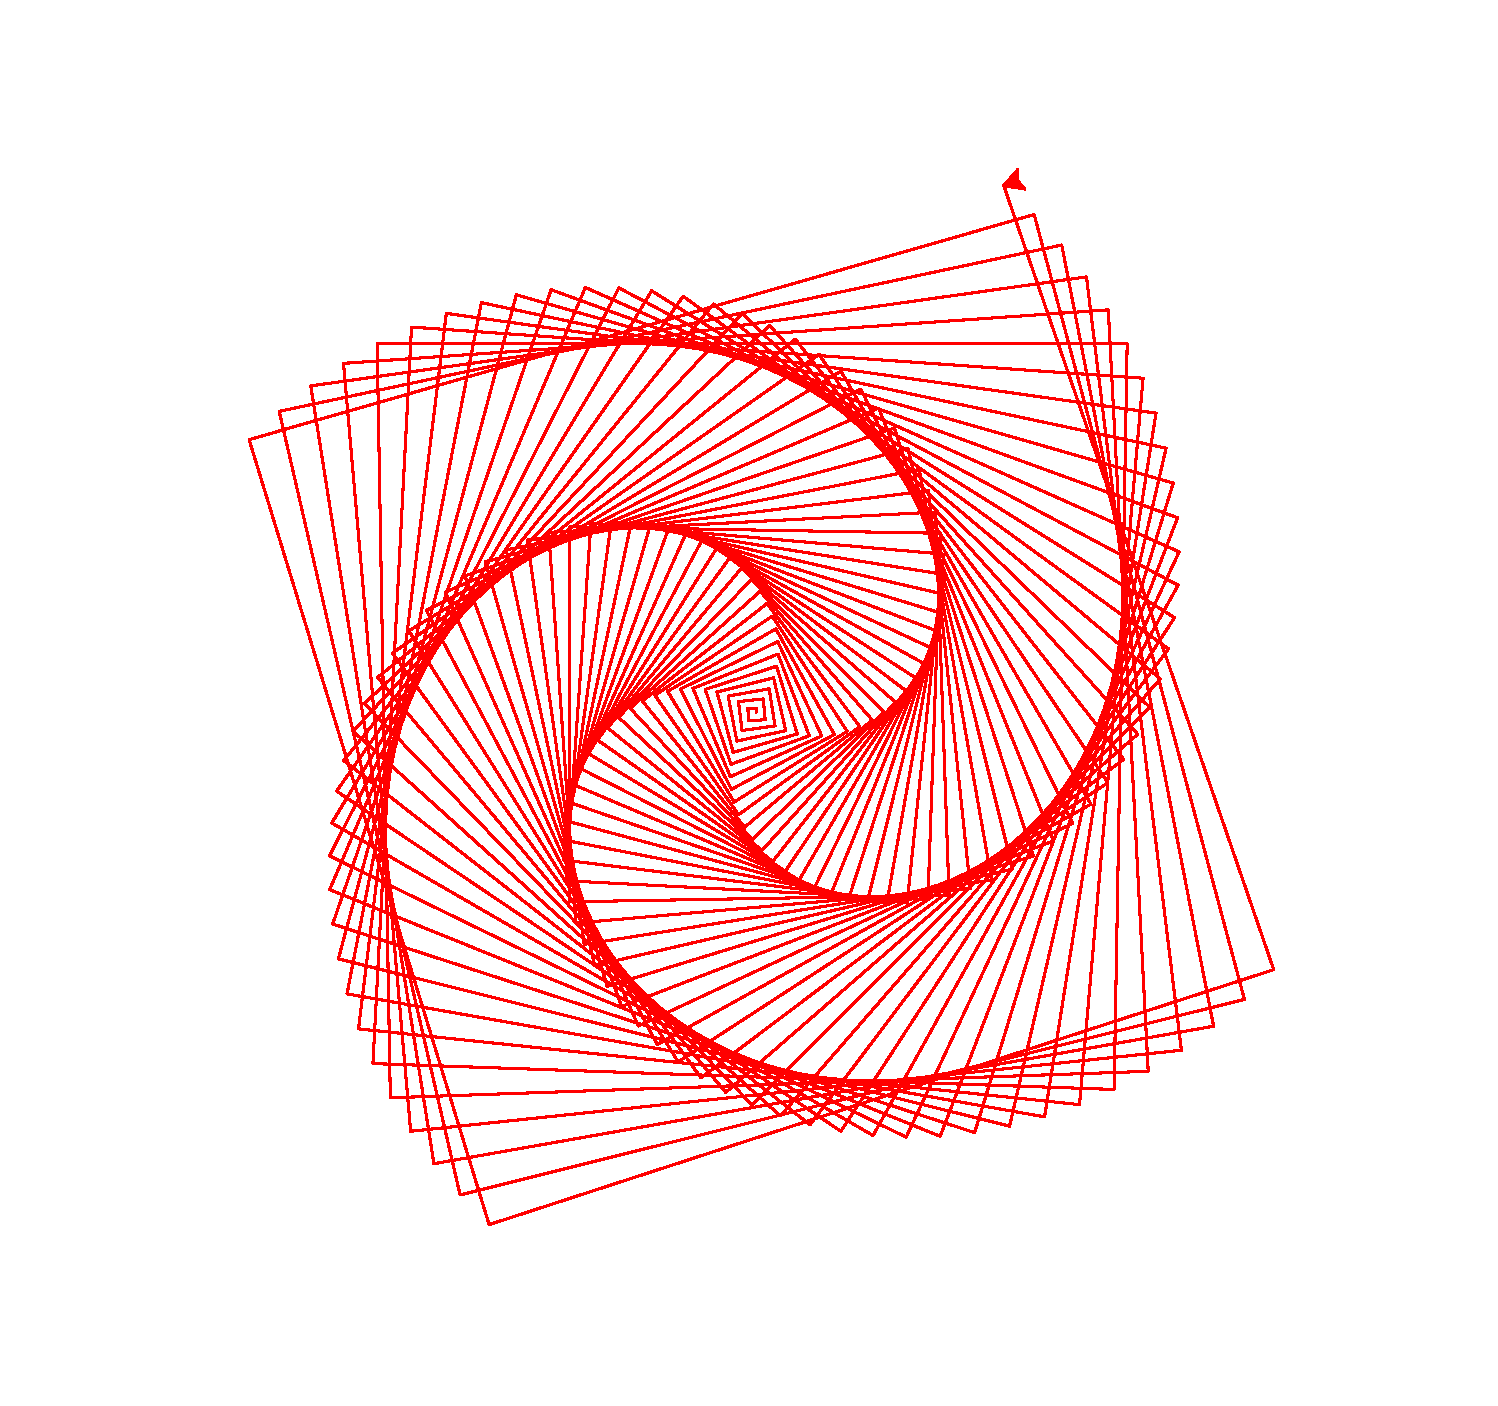
\includegraphics[clip,trim=70 70 70 70, width=\textwidth]{code/Square_Spiral_3.pdf}};
}

Try replacing ``red'' with another common colour, like ``blue'' or ``green'', and run the program again. You can use hundreds of different colours with the Turtle library, including some weird ones like ``salmon'' and ``lemon chiffon''. Or, like we did last week, you can defined your own colours by saying how much red , green and blue is to be mixed together.

Making the whole spiral a different colour is a nice step, but what if we wanted to make each side a different colour? That's going to take a few more changes to our program.

\subsection{A four-colour spiral}

Let's think through the --- that is, the set of steps --- that will turn our one-colour spiral into a four-colour spiral. The complete code is on the next page but try to write this yourself with following the structure given below 
\begin{itemize}
\item Import the turtle module and set up a turtle.
\item Tell the computer which colours we'd like to use.
\codeonly{}{7}{7}{code}{Color_Square_Spiral.py}

\item Set up a loop to draw 200 lines in our spiral.
\item Pick a different pen colour for each side of the spiral.
\codeonly{}{10}{10}{code}{Color_Square_Spiral.py}

The ``\%'' computes the remainder when we divide x by four so when 

\centerline{
\begin{tabular}{lccccccccccccccc}
	\text{x variable}  &=& 0 & 1 & 2 & 3 & 4 & 5 & 6 & 7 & 8 & 9 &10 & 11 & \ldots \\
	\text{ \code{x\%4}} &=& 0 & 1 & 2 & 3 & 0 & 1 & 2 & 3 & 0 & 1 & 2 & 3 & \ldots 
\end{tabular}}
\item Move the turtle forward to draw each side.
\item Turn the turtle left to get ready to draw the next side.
\end{itemize}
\begin{itemize}

\item[\todoSymbol] \color{todo}
Create a new file with the following code and save as \code{Color_Square_Spiral.py}.
\end{itemize}

\codeandoutput{title={\code{Color_Square_Spiral.py}}}{1}{200}{code}{Color_Square_Spiral.py}{%
	\centering	
	\tikz\node[fill=white]{
	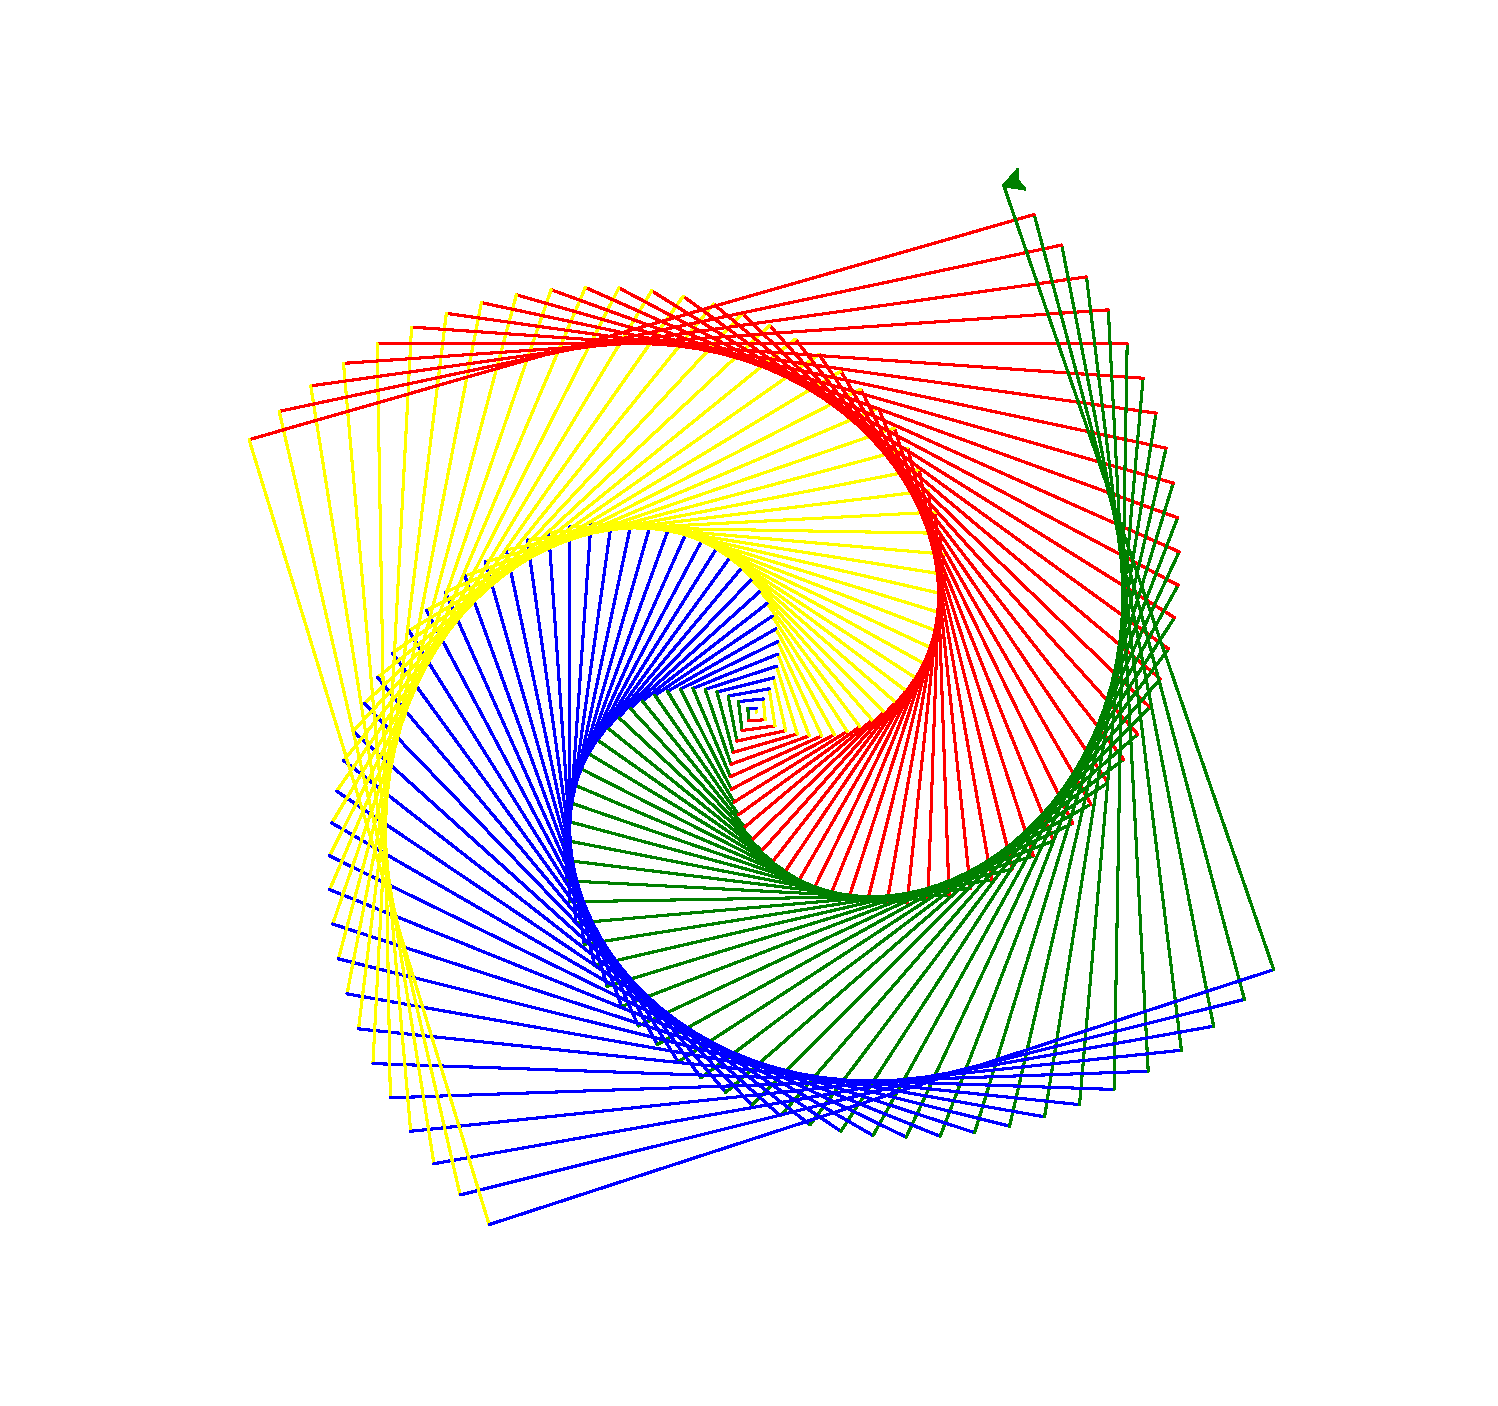
\includegraphics[clip,trim=70 70 70 70, width=\textwidth]{code/Color_Square_Spiral.pdf}};
}

\subsection{Changing the background colour}

Let's mix things up a bit again to see if we can make the generated image better.  One thing that we could do is to change the background to a dark colour so that the colours will have better contrast.

\begin{itemize}
\item[\todoSymbol] \color{todo}
Save \code{Color_Square_Spiral.py} as \code{Color_Square_Spiral_2.py}  and insert lines 7 and 8 as shown below.
\end{itemize}

\codeandoutput{title={\code{Color_Square_Spiral_2.py}}}{1}{200}{code}{Color_Square_Spiral_2.py}{%
	\centering	
	\tikz\node[fill=black]{
	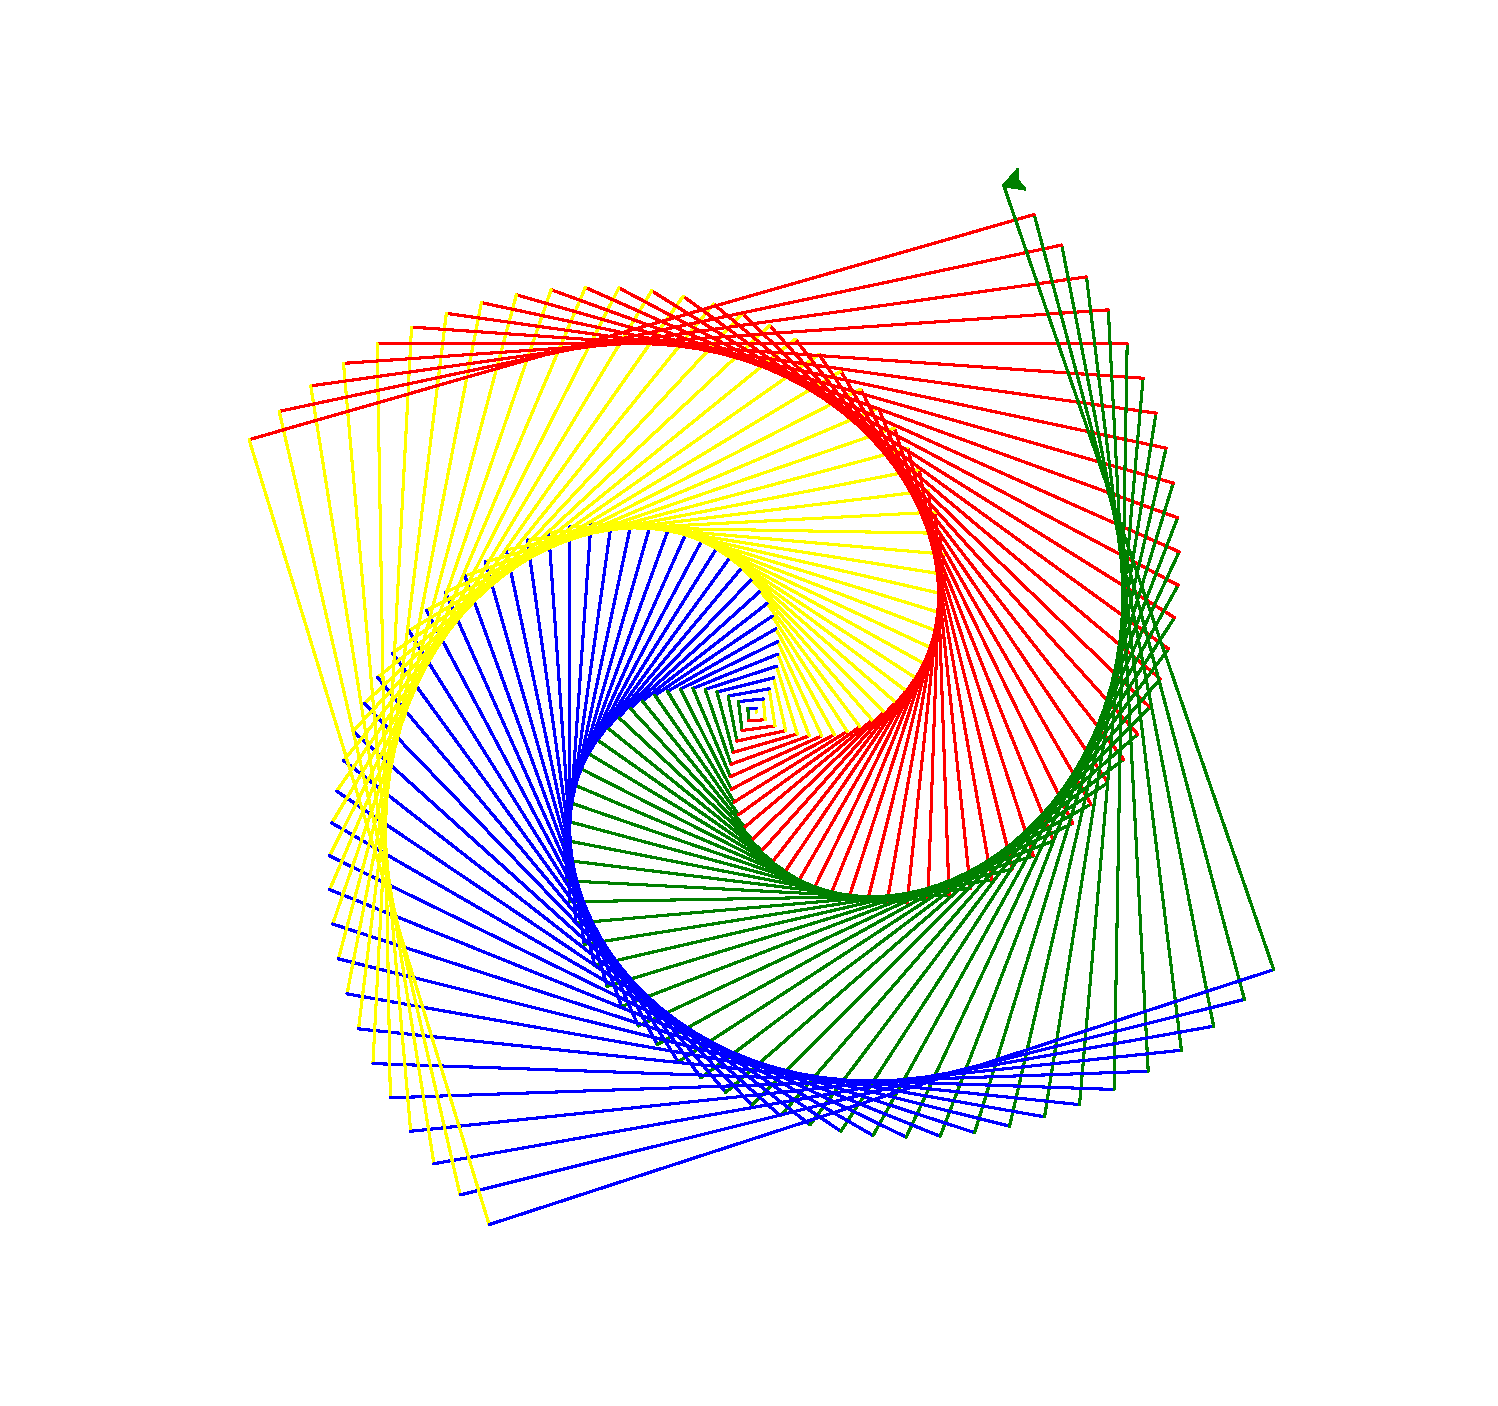
\includegraphics[clip,trim=70 70 70 70, width=\textwidth]{code/Color_Square_Spiral_2.pdf}};
}

We have inserted two lines:
\begin{itemize}
\item[{\smaller line 7:}] Gives us access to the \code{window} within which out turtle, \code{bob} lives.
\item[{\smaller line 8:}] We set the background colour using command \code{bgcolor}.
\end{itemize}

%\centerline{
%\tikz\node[draw,fill=red!5,drop shadow] {This is a small bug in the program that generates these worksheets. This does not capture the background colour 
%};
%}

\subsection{How many sides?}

OK, we have done a lot with spirals and it is time to move to something new. Before we do that, have a look at the following program 
 
\begin{itemize}
\item[\todoSymbol] \color{todo}
Create a new file with the following code and save as \code{Color_Spiral.py}.

Change the value of \code{sides} to get the diagram shown.
\end{itemize}

\codeandoutput{title={\code{Color_Spiral.py}}}{1}{200}{code}{Color_Spiral.py}{%
	\centering	
	\tikz\node[fill=black,align=center]{
	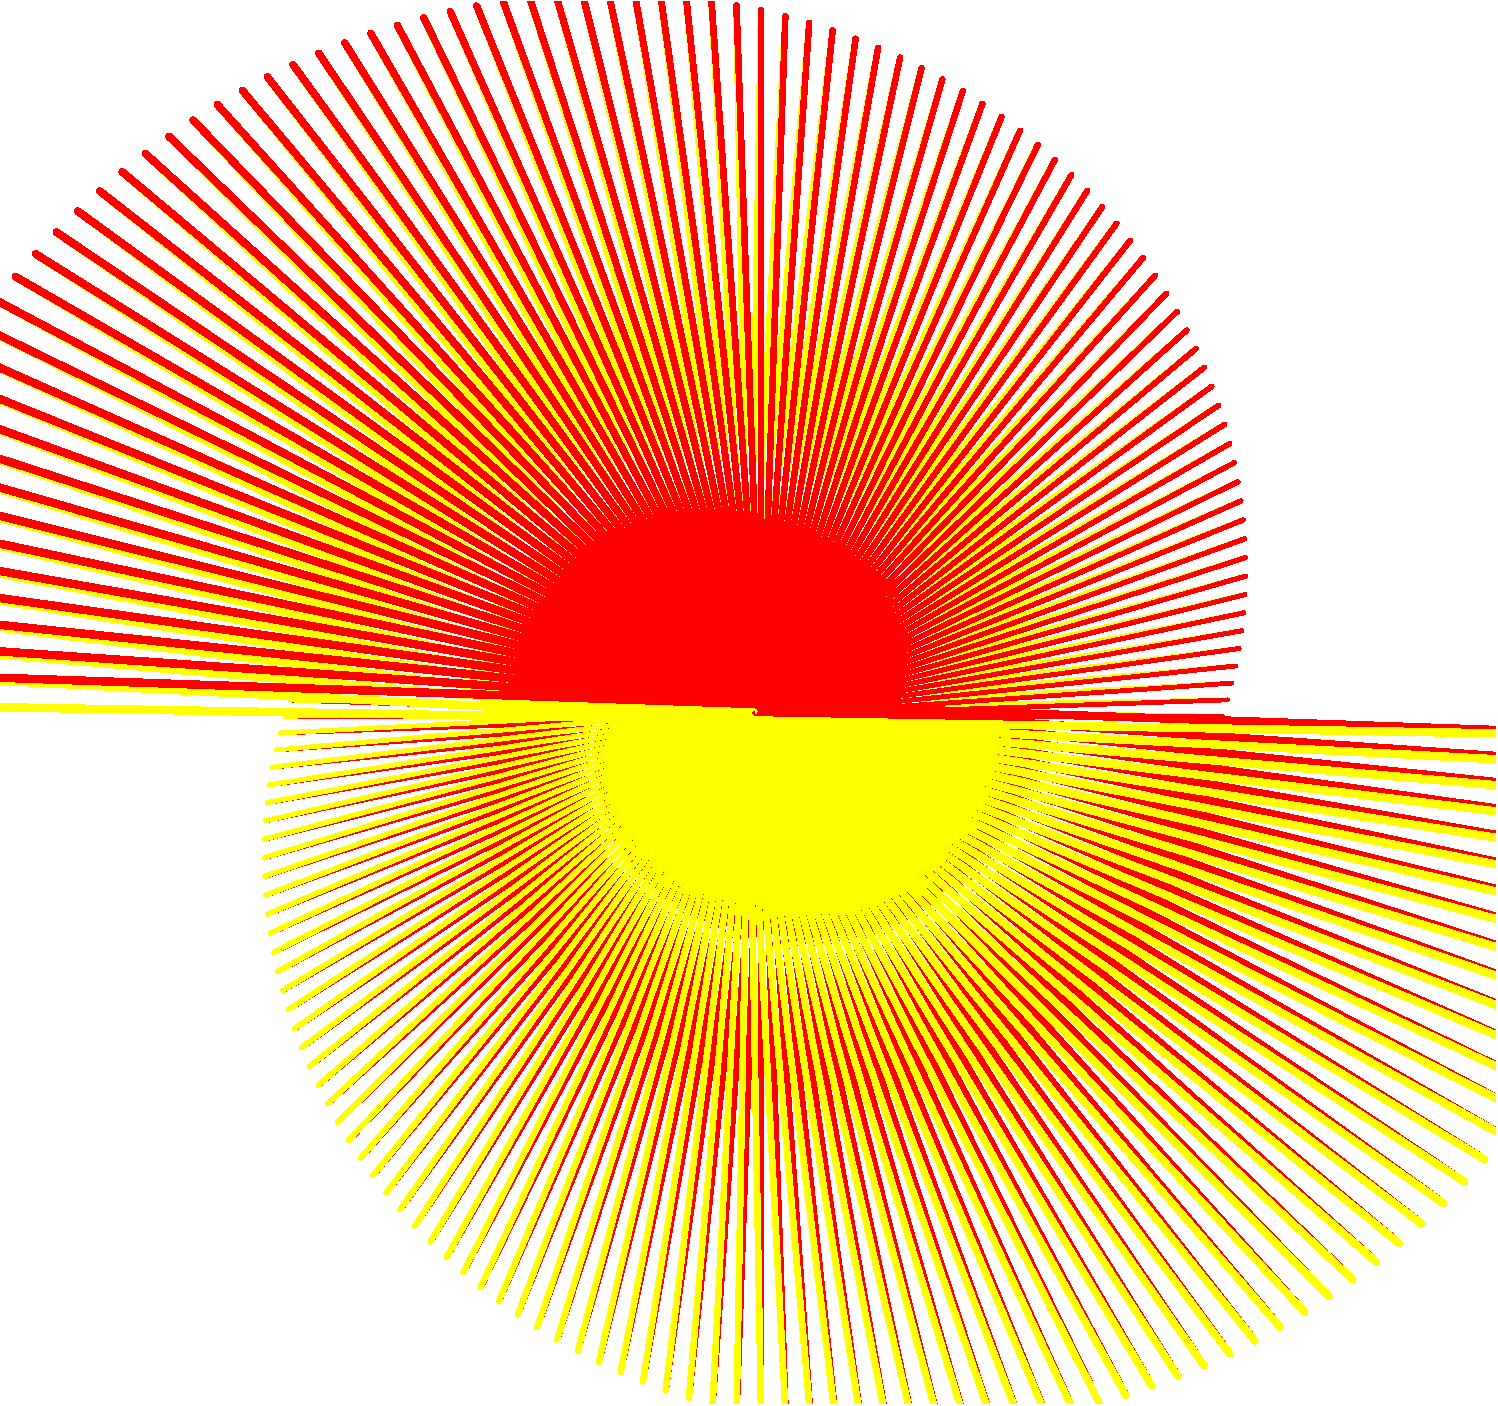
\includegraphics[clip,trim=0 0 0 0, width=\textwidth]{code/Color_Spiral_a.pdf}\\
	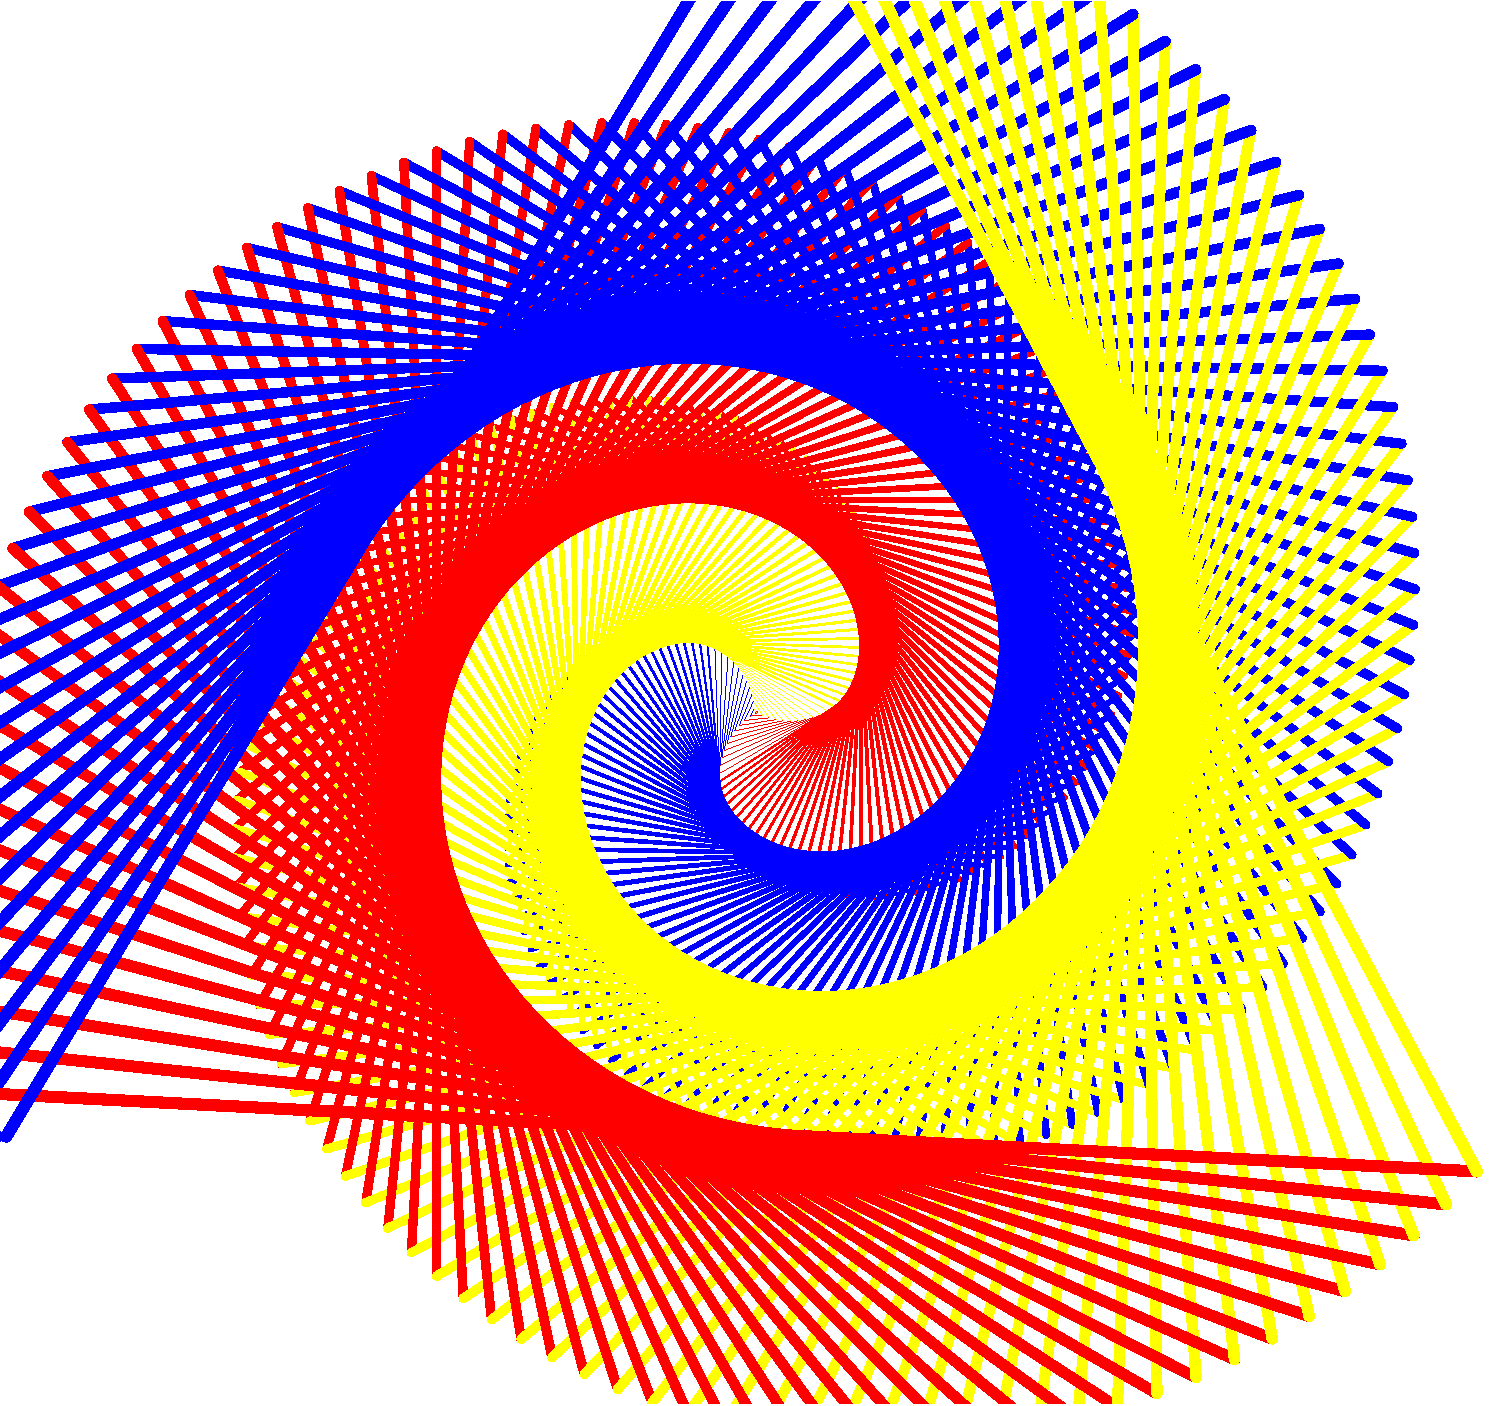
\includegraphics[clip,trim=0 0 0 0, width=\textwidth]{code/Color_Spiral_b.pdf}\\
	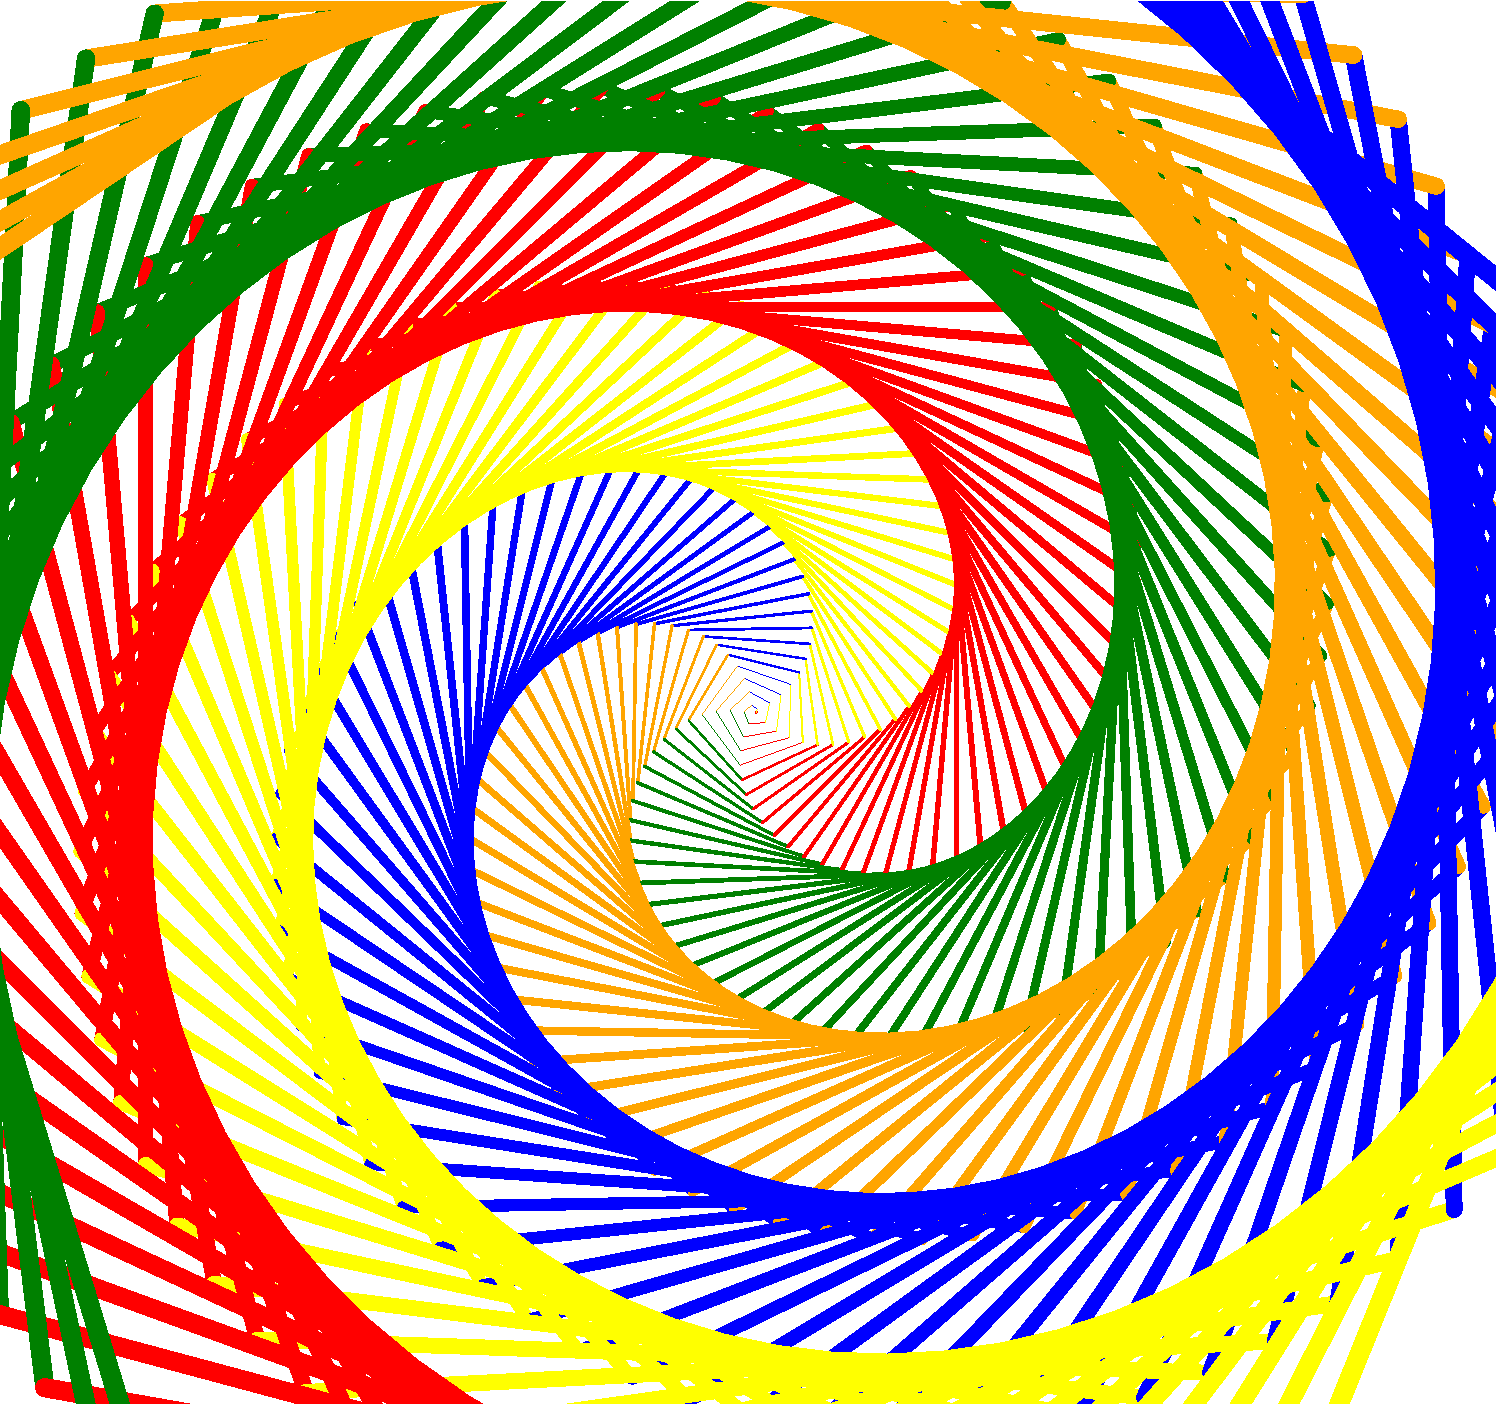
\includegraphics[clip,trim=0 0 0 0, width=\textwidth]{code/Color_Spiral_c.pdf}
	};
}

\clearpage

%\section{To Fill or Not Fill --- That is the Question}\label{sec:fill}
\section{Why are my Shapes so Empty?}\label{sec:fill}

Remember our first turtle program that just drew a square:

\codeandoutput{title={\code{Square.py}}}{1}{200}{code}{Square.py}{%
	\centering	
	\tikz\node[fill=white]{
	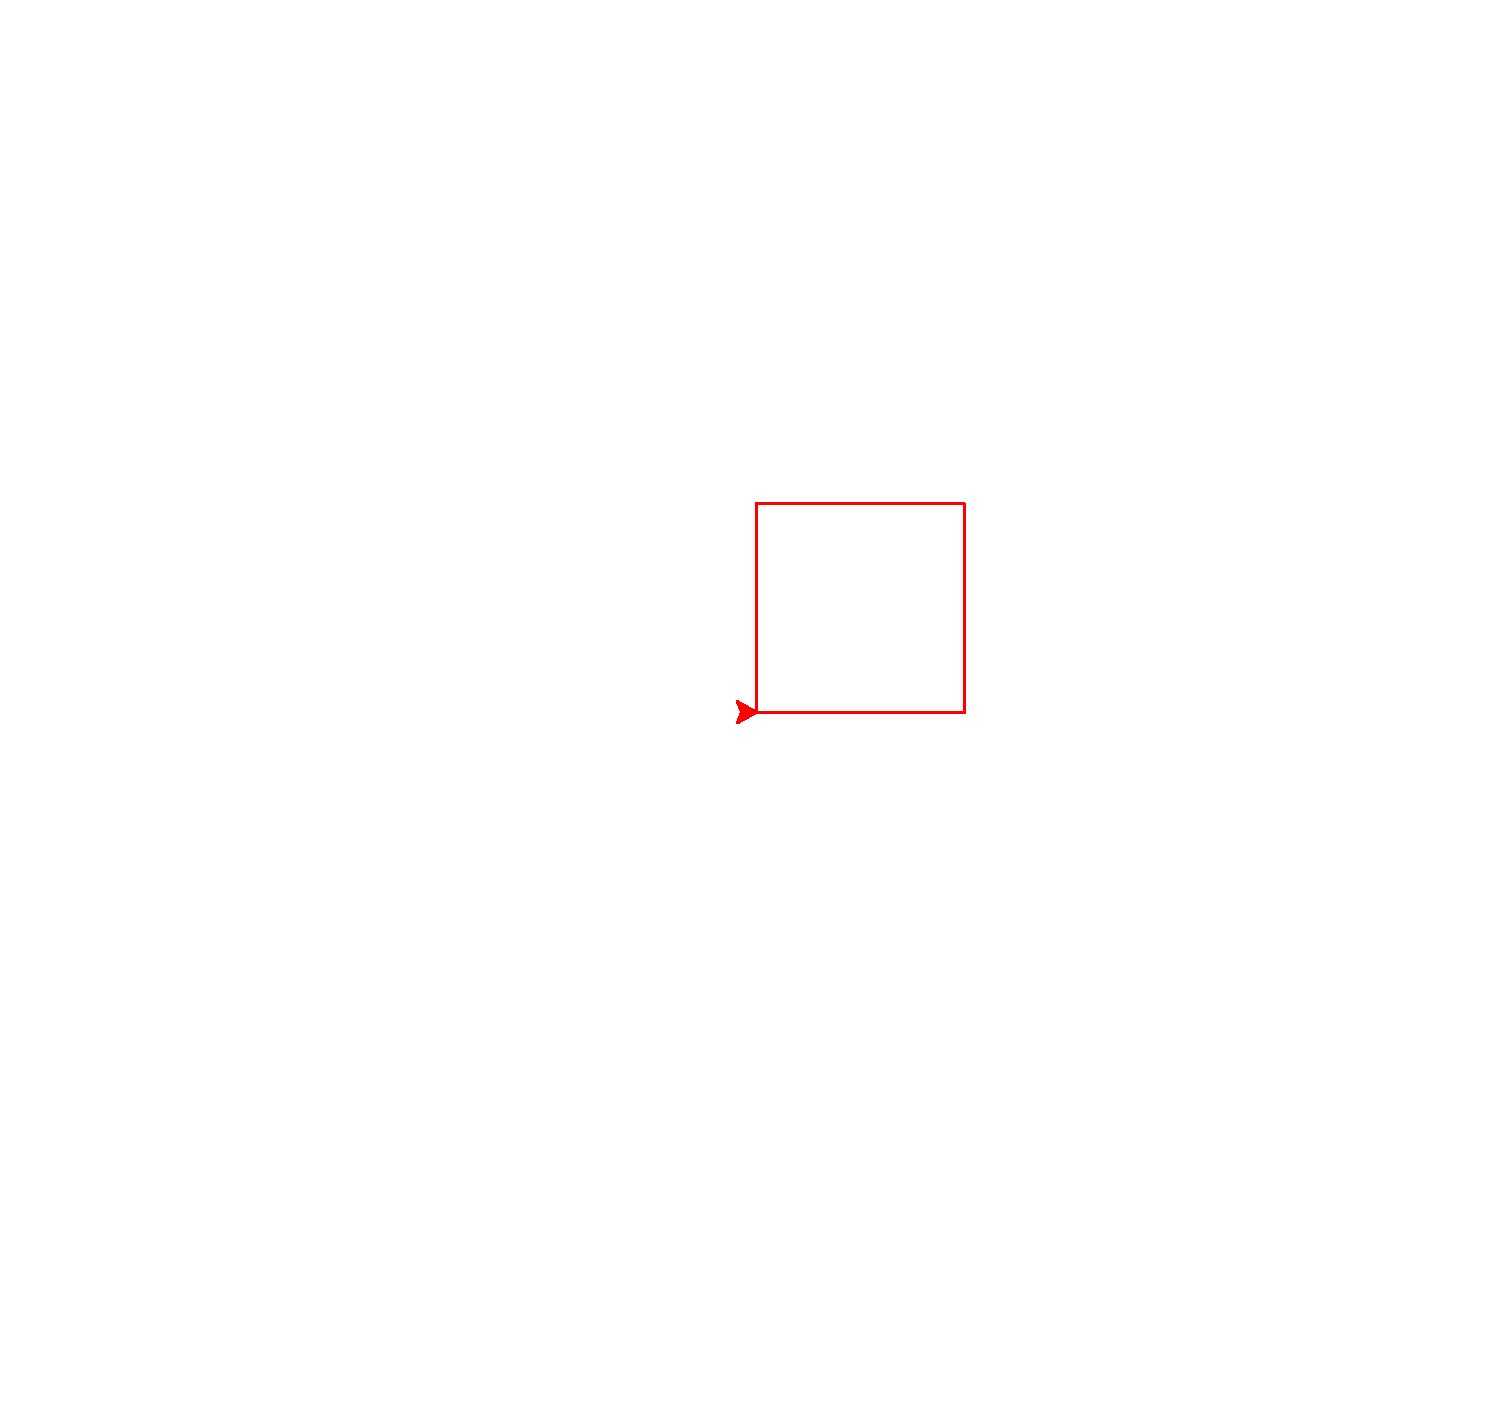
\includegraphics[clip,trim=70 70 70 70, width=\textwidth]{code/Square.pdf}};
}

It would be nice if we could fill this square, or any shape, with a colour of our choice. We can 

\begin{itemize}
\item[\todoSymbol] \color{todo}
Create a new file with the following code and save as \code{Square_Fill.py}.
\end{itemize}

\codeandoutput{title={\code{Square_Fill.py}}}{1}{200}{code}{Square_Fill.py}{%
	\centering	
	\tikz\node[fill=white]{
	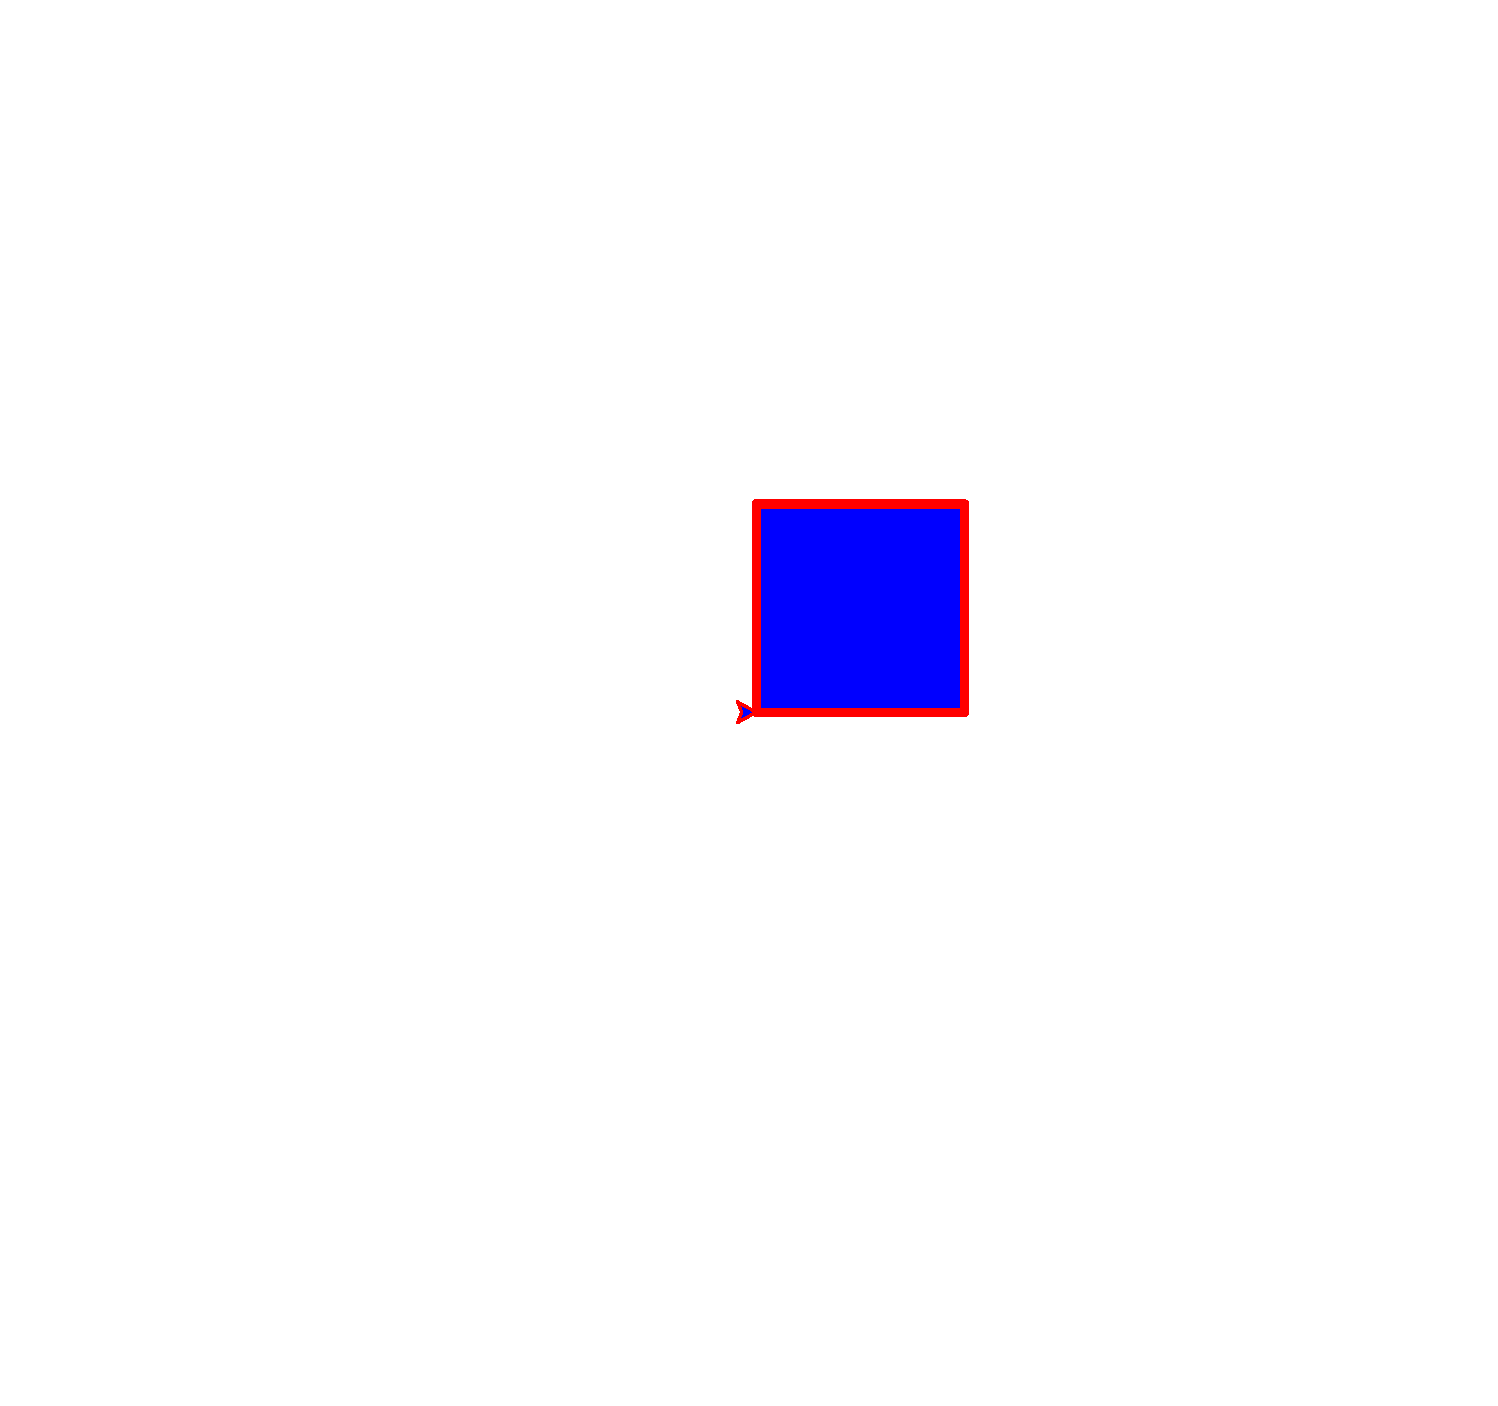
\includegraphics[clip,trim=70 70 70 70, width=\textwidth]{code/Square_Fill.pdf}};
}


\begin{itemize}
\item We set the fill colour using the command \code{fillcolor}.
\item Note: I increased the line width, using the command \code{width}, so that it was easier to see the outline.
\end{itemize}

\clearpage

\section{Exercises}

Try to create each of the following diagrams. All of the diagrams can be draw using the turtle commands that we covered this week and last week.

\begin{center}
\begin{tabular}{cccc}

\code{circles} & \code{chess} &  \code{more_circles}  \\
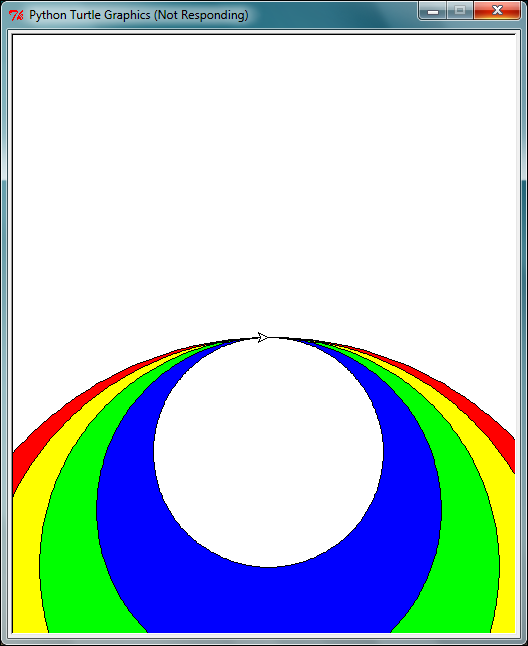
\includegraphics[clip,trim=20 20 20 100, width=5cm]{circles} &
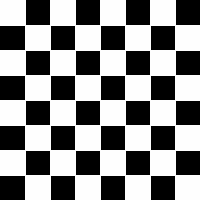
\includegraphics[width=5cm]{chess.png} &  
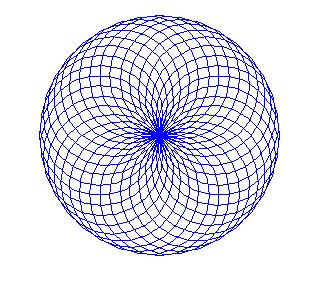
\includegraphics[clip,trim=0 0 0 0, width=5cm]{circles_2}
  \\[30pt]
  
\code{face} & \code{party} &  \code{city}  \\
 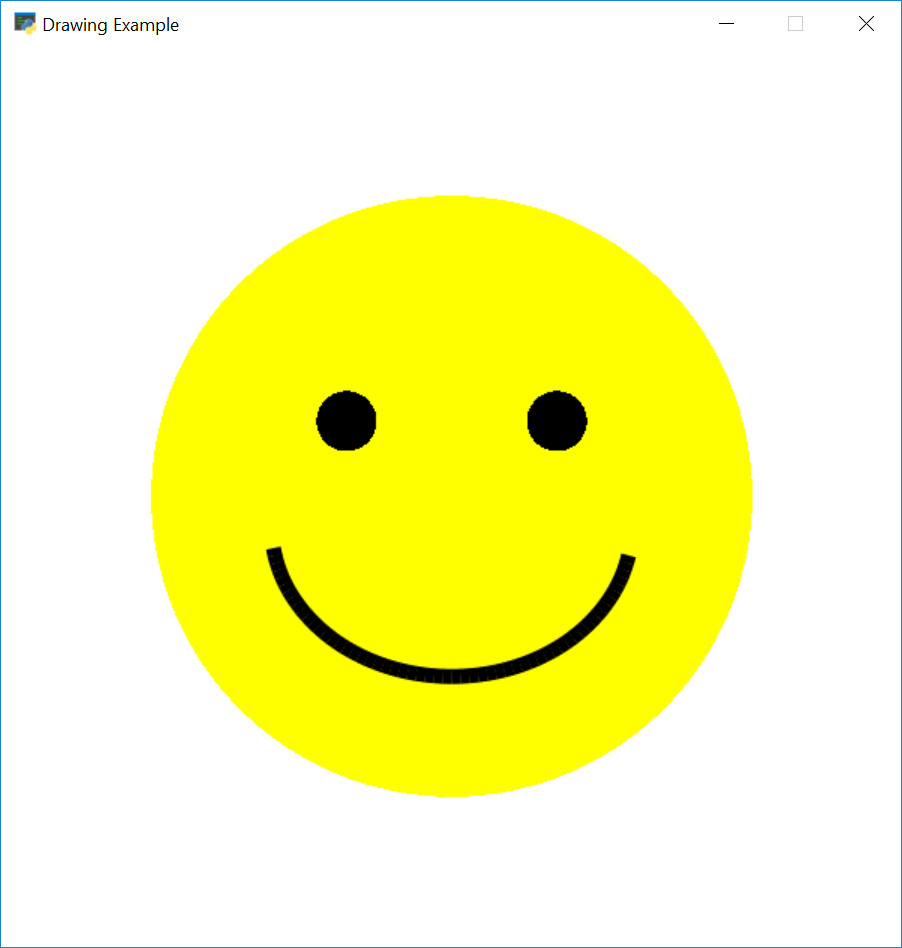
\includegraphics[clip,trim=20 20 50 20, width=5cm]{face.png} &
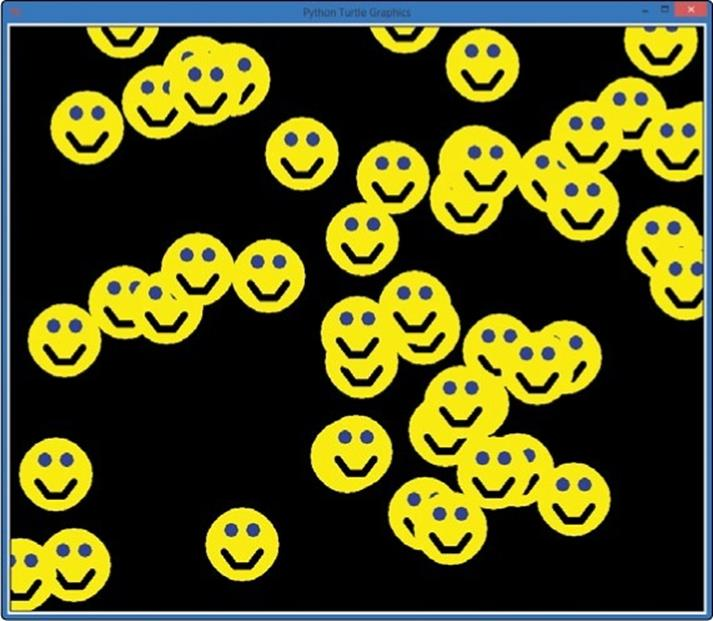
\includegraphics[clip,trim=20 20 50 20, width=5cm]{faces.png} &
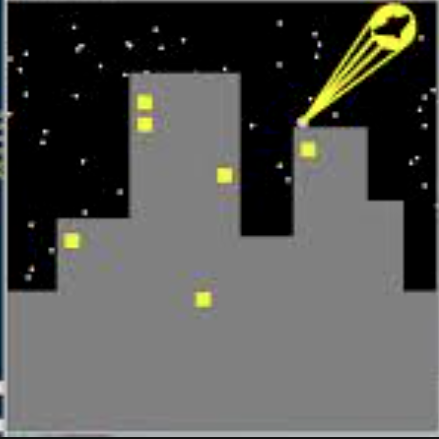
\includegraphics[width=5cm]{batman.png} & 
\\[30pt]
%
\code{house_outline} & \code{house_small} & \code{house_big}\\
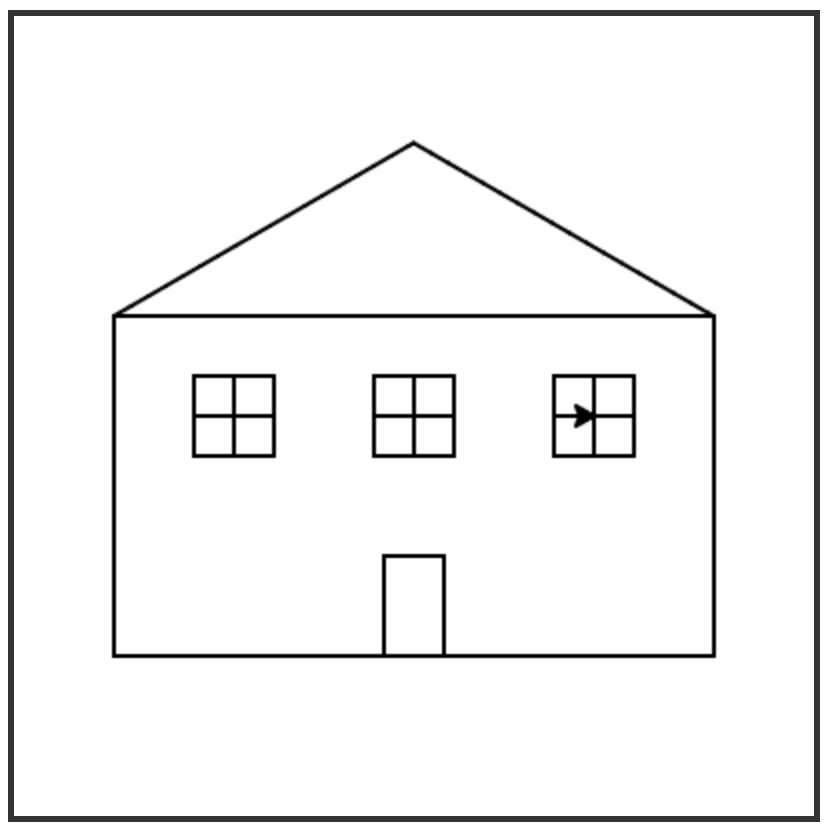
\includegraphics[width=5cm]{house_0.png} &
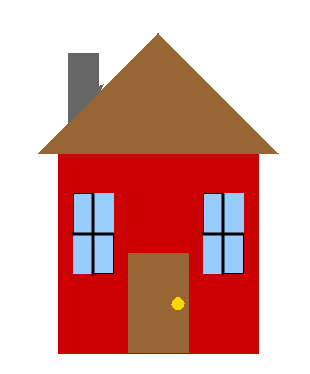
\includegraphics[width=5cm]{house_1.png} &
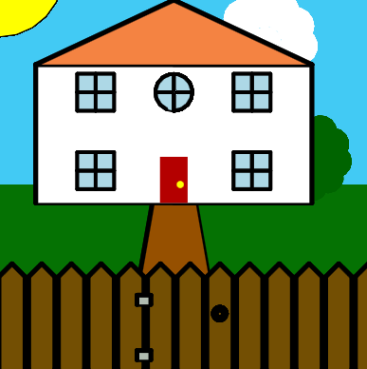
\includegraphics[width=5cm]{house_2.png} 
\end{tabular}
\end{center}

\end{document}
